\section{Introduzione all'esperienza}
Vogliamo studiare le caratteristiche del decadimento gamma di diversi isotopi radioattivi e dell'interazione tra raggi gamma e materia. 
L'interesse nello studio deriva dai risultati ottenuti che forniscono informazioni utili sulla struttura nucleare atomica e sui numeri quantici ad essa relativi.
Per effettuare uno studio precisoi useremo dei rivelatori \ce{NaI(Tl)} letti da un fotomoltiplicatore.

\subsection{sezioni}
\begin{itemize}
    \item proprietà della catena elettronica di misura?
    \item calibrazione multicanale
    \item studio di sorgenti \ce{^137Cs} \ce{^60Co} \ce{^22Na} \ce{^57Co}
    \item identificazione elementi radioattivi in rocce e fondo ambientale (analisi gamma)
    \item risoluzione del rivelatore, misura FWHM di \ce{^137Cs} \ce{^60Co} \ce{^22Na}
    \item misura relativa e assoluta dell'attività di una sorgente
    \item misura assorbimento gamma nel \ce{Pb}, determinazione coeff. $\mu$ assorb. massa
    \item effetti di somma nello spettro di \ce{^60Co} (struttura livelli nucleo figlio)

\end{itemize}

\section{postazione A e apparecchiatura}

La postazione usa come rivelatore un cristallo di \ce{NaI(Tl)} di diametro $ 2^{"} = 50.8 mm $ letti da fotomoltiplicatori. Nello specifico la nostra posizione usa moduli NIM per alimentare i fotomoltiplicatori e l'elettronica di amplificazione, questa configurazione ci permette di studiare il segnale del fotomoltiplicatore con un oscilloscopio.
\begin{center}
    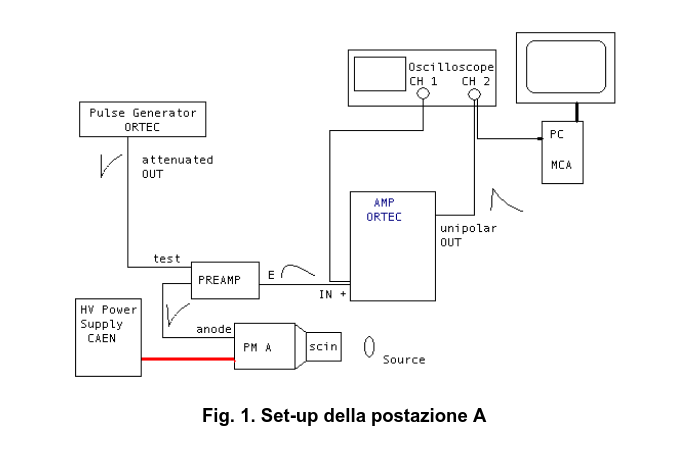
\includegraphics[scale=0.5]{images/setup_A}
\end{center}

Attenzione:
\begin{itemize}
    \item Manipolare le sorgenti con le apposite pinzette e lasciare le sorgenti nella cassetta di piombo per tutta l'esperienza
    \item ogni rivelatore ha una tensione massima (HV) da rispettare per mantenere l'integrità dei componenti (impostare a 0 prima di uscire dal programma di acquisizione)
    \item lasciare invariata la posizione delle mattonelle di piombo (tossico per ingestione)
\end{itemize}
